% Slide 19: Next Steps
\begin{frame}{Next Steps}
    \framesubtitle{Path Forward}

    \begin{center}
        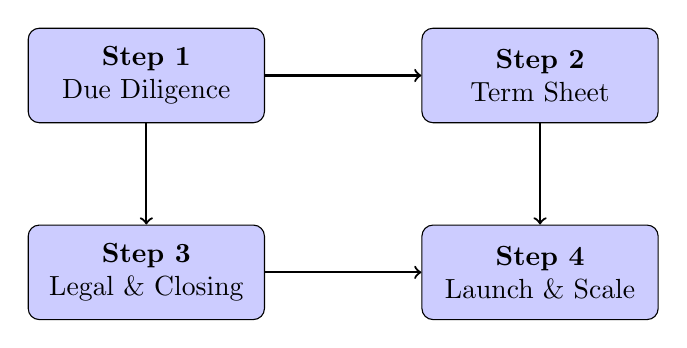
\begin{tikzpicture}[
            box/.style={rectangle,draw,fill=blue!20,rounded corners,minimum width=3cm,minimum height=1.2cm,align=center},
            node distance=2.5cm
        ]
            \node[box] (step1) {\textbf{Step 1}\\Due Diligence};
            \node[box,right of=step1,node distance=5cm] (step2) {\textbf{Step 2}\\Term Sheet};
            \node[box,below of=step1] (step3) {\textbf{Step 3}\\Legal \& Closing};
            \node[box,right of=step3,node distance=5cm] (step4) {\textbf{Step 4}\\Launch \& Scale};

            \draw[->,thick] (step1) -- (step2);
            \draw[->,thick] (step2) -- (step4);
            \draw[->,thick] (step1) -- (step3);
            \draw[->,thick] (step3) -- (step4);
        \end{tikzpicture}
    \end{center}

    \vspace{0.5cm}

    \begin{columns}[t]
        \begin{column}{0.3\textwidth}
            \textbf{Immediate Actions:}
            \begin{enumerate}
                \item Schedule follow-up meeting
                \item Share detailed financial model
                \item Provide customer references
                \item Arrange product demo
                \item Share data room access
            \end{enumerate}
        \end{column}

        \begin{column}{0.3\textwidth}
            \textbf{Timeline:}
            \begin{itemize}
                \item \textbf{Week 1-2:} Due diligence
                \item \textbf{Week 3:} Term sheet negotiation
                \item \textbf{Week 4-6:} Legal documentation
                \item \textbf{Week 7:} Closing
                \item \textbf{Week 8+:} Execution
            \end{itemize}
        \end{column}
    \end{columns}
\end{frame}
